\documentclass[a4paper, 11pt]{report}

\usepackage[utf8]{inputenc}
\usepackage[T1]{fontenc}
\usepackage{amsfonts}
\usepackage{amsmath}
\usepackage{amsthm}
\usepackage{ccaption}
\usepackage{caption}
\usepackage{chngcntr}
\usepackage{enumitem}
\usepackage{fancyhdr}
\usepackage{float}
\usepackage{gensymb}
\usepackage{geometry}
\usepackage{graphicx}
\usepackage{hyperref}
\usepackage{lastpage}
\usepackage{layout}
\usepackage{multicol}
\usepackage{multirow}
\usepackage[final]{pdfpages} 
\usepackage{pstricks}
\usepackage{siunitx}
\usepackage{soul}
\usepackage{titlesec}
\usepackage{ulem}
\usepackage{url}
\usepackage{xcolor}
\usepackage{wrapfig}
\usepackage{listings}
\lstnewenvironment{c++}[1][]{
\lstset{
upquote=true,
columns=flexible,
basicstyle=\ttfamily,
language=c++,
keywordstyle=\color{blue},
commentstyle=\color{gray},
breaklines,
breakindent=1.5em,
xleftmargin=2em,
xrightmargin=2em,
frame=single,
rulecolor=\color{orange},
backgroundcolor=\color{orange!5},
}}{}

\geometry{hmargin=2.75cm,vmargin=2.5cm}

\fancyhf{}

\lhead{{\ifthenelse{\value{page}=1}{}{Ricossa Sergio}}}

\chead{{%sinon
\ifthenelse{\value{page}=1}{%page 1
}{%sinon
Counterproof of the Daddy conjecture}}}
%veuillez mettre  le nom de l'expérience nom ci-dessus !!!

\rhead{{%sinon
\ifthenelse{\value{page}=1}{%page 1
}{%sinon
\today}}}
\lfoot{\ifthenelse{\value{page}=1}{%page 1
}{%sinon
}}
\rfoot{\ifthenelse{\value{page}=1}{%page 1
}{%sinon
}
}
\cfoot{\ifthenelse{\value{page}=1}{%page 1
\thepage \hspace{1pt} / \pageref{LastPage}}{%sinon
\ifthenelse{\value{page}=0}{0
}{%sinon
\thepage \hspace{1pt} / \pageref{LastPage}}}}
\setcounter{page}{1}
\date{\Large{ \today}}

\author{\Large{Ricossa Sergio}}

\renewcommand{\headrulewidth}{
\ifnum\value{page}=1
    0pt
  \else
    \ifnum\value{page}=0
    0.5pt
  \else
    0.5pt
  \fi
  \fi}

\pagestyle{fancy}


%la définition ci dessous permet d'avoir accès aux sous-sous-soussections

\titleclass{\subsubsubsection}{straight}[\subsection]

\newcounter{subsubsubsection}[subsubsection]
\renewcommand\thesubsubsubsection{\thesubsubsection.\arabic{subsubsubsection}}
\renewcommand\theparagraph{\thesubsubsubsection.\arabic{paragraph}} % optional; useful if paragraphs are to be numbered

\titleformat{\subsubsubsection}
  {\normalfont\normalsize\bfseries}{\thesubsubsubsection}{1em}{}
\titlespacing*{\subsubsubsection}
{0pt}{3.25ex plus 1ex minus .2ex}{1.5ex plus .2ex}

\makeatletter
\renewcommand\paragraph{\@startsection{paragraph}{5}{\z@}%
  {3.25ex \@plus1ex \@minus.2ex}%
  {-1em}%
  {\normalfont\normalsize\bfseries}}
\renewcommand\subparagraph{\@startsection{subparagraph}{6}{\parindent}%
  {3.25ex \@plus1ex \@minus .2ex}%
  {-1em}%
  {\normalfont\normalsize\bfseries}}
\def\toclevel@subsubsubsection{4}
\def\toclevel@paragraph{5}
\def\toclevel@paragraph{6}
\def\l@subsubsubsection{\@dottedtocline{4}{7em}{4em}}
\def\l@paragraph{\@dottedtocline{5}{10em}{5em}}
\def\l@subparagraph{\@dottedtocline{6}{14em}{6em}}
\makeatother

\setcounter{secnumdepth}{4}
\setcounter{tocdepth}{4}




%Vous pouvez choisir les couleurs de vos titres (de 0 à 1)
\titleformat{\section}{\color[rgb]{0,0,0.5}\Large\bfseries}{\color[rgb]{0,0,0.5}\thesection}{1em}{}

\titleformat{\subsection}{\color[rgb]{0,0,0.6}\large\bfseries}{\color[rgb]{0,0,0.6}\thesubsection}{1em}{}

\titleformat{\subsubsection}{\color[rgb]{0,0,0.77}\normalsize\bfseries}{\color[rgb]{0,0,0.77}\thesubsubsection}{1em}{}

\titleformat{\subsubsubsection}{\color[rgb]{0,0,0.9}\normalsize\bfseries}{\color[rgb]{0,0,0.9}\thesubsubsubsection}{1em}{}

\newtheorem{definition}{Definition}
\newtheorem{theorem}{Theorem}

\begin{document}

\title{\Huge{\underline{Counterproof of the Daddy conjecture}}}

\maketitle
\thispagestyle{fancy}
\newpage
\section{Introduction}
	In the "Papa Flammy's advent Calendar" youtube series, Flammable Math introduced an interesting conjecture about a particular property of the number 52 presented in the video at the following link: \url{https://www.youtube.com/watch?v=4Uqd9QexPuA}. He conjectured that this property happens infinitely many times among integers.
	
	In this paper, combining analytical and numerical methods, we disprove this conjecture by showing 52 is unique in exhibiting that property. We also prove a more general statement.
	
	This proof is complemented by numerical calculations. All the important files can be found in the following Github repository: \url{https://github.com/sbacco/daddynessK}.

\section{Statement of the conjecture}

	First off, some definitions:
	\begin{definition}
		Let $n\in\mathbb{N}$ such that $n = \sum_{i=1}^Nd_i\cdot10^{N-i}$.
		
		\begin{itemize}
			\item The \emph{digit sum} of $n$ is: $S(n):=\sum_{i=1}^Nd_i$
			\item The \emph{alternate digit sum} of $n$ is: $A(n):=-\sum_{i=1}^N(-1)^id_i$
			\item The \emph{concatenation} $conc(n_1,n_2,n_3,\dots)$ of a list of numbers $n_i$ is the number obtained by putting the $n_i$ one after the other in base 10:
		\end{itemize}
	\end{definition}

	We write: $conc(n_1,n_2,n_3,\dots) =: n_1\circ n_2\circ n_3\circ\dots$
			
	For example: $12\circ4\circ123=124123$
	
	\begin{definition}
		Let $n\in\mathbb{N}$. Let: $\sigma:=S(n)+A(n)$. 
		
		Let $\sigma=\prod_{i=1}^\xi p_i$ the prime factors decomposition of $\sigma$, where $p_i$ are ordered from smallest to greatest.
		
		$n$ is said to be \emph{pseudo-daddy} if:
		For some permutation $j(i)$ of the indices, one has:
		$$n=p_{j(1)}\circ p_{j(2)}\circ\dots\circ p_{j(\xi)}$$
		
	\end{definition}
	
	Although $A$ can be negative, it's easy to check that $\sigma$ is always positive and divisible by $2$. One way to obtain it is to sum up every two digits of $n$ and multiply by $2$.
		
	For example: $n:=1234\Rightarrow \sigma=2(1+3)=8$
	
	Finally:
	
	\begin{definition}
		Let $n\in\mathbb{N}$.
		
		$n$ is said to be \emph{daddy} if it is pseudo-daddy and if both $S(n)$ and $A(n)$ are primes.
		
	\end{definition}
	
	The theorem we will prove is the following:
	
	\begin{theorem}
		There are exactly $5$ pseudo-daddy numbers:
		$22,32,52,72,222$
		
		There is only one daddy number: $52$
	\end{theorem}
	
	This is proof that the \emph{Daddy conjecture} that Flammable Math proposed in his video is wrong, as he proposed there are infinitely many daddy numbers.
	
	It's easy to show that the listed numbers are effectively pseudo-daddy. The second statement is also easy to prove. You can just try to evaluate $A$ and $S$ for the 5 numbers above. Only $52$ gives 2 primes.
	
	We will focus on showing the first part in this paper.

\newpage
\section{Proof of the theorem}
\begin{proof}
	A crucial component of the proof is the program provided with it. We compiled a C++ program that finds through brute force every pseudo-daddies smaller than 10 Million. As one can verify, we immediately find the above mentioned numbers, but no other number.
	
	We therefore just have to show that there are no pseudo-daddies greater than 10 Million.
	
	Let's choose $n$ to be some N-digits pseudo-daddy number, with:
	$$n:=d_1\circ d_2\circ\dots\circ d_N \text{ ; } d_i\in\{0,1,\dots,9\}$$
	We also write, for short:
	$$S,A:=S(n),A(n)$$
	We define the prime factors expansion:
	$$\sigma=2\prod_{i=1}^\xi p_i$$
	where we separated the factor of $2$ from the rest, since we know $\sigma$ is even.
	
	One has that:
	\begin{itemize}
		\item If $N$ is even: $\sigma=2\sum_{i=1}^{N/2}d_{2i-1}\leq2\cdot(N/2)\cdot9$
		\item If $N$ is odd: $\sigma=2\sum_{i=1}^{(N+1)/2}d_{2i-1}\leq(N+1)\cdot9$
	\end{itemize}
	
	Indeed, as we vaguely discussed above, adding $A$ to $S$ just takes away the even $d_i$'s and doubles the odd ones. So:
	
	\begin{equation}
		\sigma=2\prod_{i=1}^\xi p_i\leq9(N+1)
		\label{ineq1}
	\end{equation}
	
	Moreover:
	$$2\prod_{i=1}^\xi p_i\geq2\cdot2^{\xi}$$
	Since prime numbers are all greater than $2$.
	
	So, sandwiching $\sigma$ we get that:
	\begin{equation}
		2^{\xi+1}\leq9(N+1)\Rightarrow\xi\leq\log_2\left(9(N+1)\right)-1
		\label{sand}
	\end{equation}

	So far, we have just done standard manipulations. Now, we use the daddyness condition:	

	Let $k_i$ be the number of digits of $p_i$:
	$$k_i\leq1+\log_{10}p_i$$
	
	For $n$ to be pseudo-daddy we need (the extra '1' comes from the factor of '2' we extracted that has to be concatenated as well):
	$$1+\sum_{i=1}^{\xi}k_i=N$$
	\begin{equation}
		\Rightarrow N\leq1+\xi+\log_{10}(\prod_{i=1}^{\xi}p_i)\leq\log_2\left(9(N+1)\right)+\log_{10}(\frac{9}{2}\left(N+1\right))=:f(N)
		\label{final}
	\end{equation}
	Where we used both (\ref{ineq1}) and(\ref{sand})
	
	We know that $N$ will 'win' over $f(N)$ as $N$ increases. We plotted the two functions on fig.\ref{plot}. They intersect only once at:
	$$N_{max}\approx7.93$$
	
	For $N> N_{max}$, the inequality (\ref{final}) is violated. Therefore, there are no pseudo-daddies with more than 7 digits.
	
	The outtake is that we only have to bruteforce our way through the first 10,000,000 positive integers to finish the proof. In this time and age, computers are much better than us at doing just that. 
	
	By running the annexed program up to $n=10,000,000$, we get all the existing pseudo-daddy numbers, listed in the theorem's statement. And that concludes the proof.
\end{proof}

\begin{figure}[htbp]
\begin{center}
	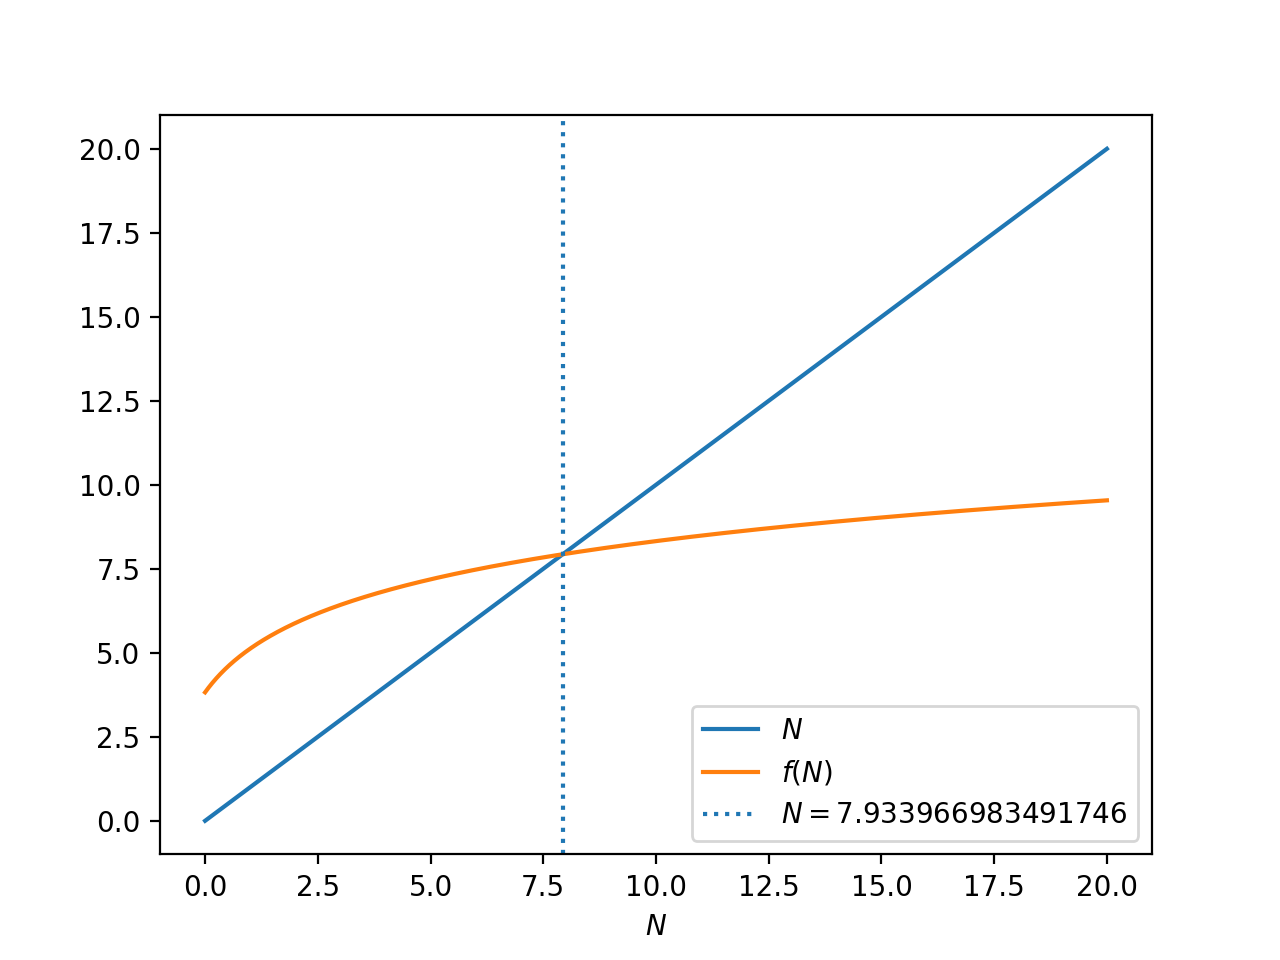
\includegraphics{plot.png}
\caption{Graphic representation of inequality (\ref{final}). The inequality is violated when the orange curves goes under the blue curve at $N\approx7.93$.}
\label{plot}
\end{center}
\end{figure}

\section{Conclusion}
	Although this is a valid proof, future improvements are still possible. The 5 only pseudo-daddy numbers are actually quite easy to guess (at least the first four) knowing that they have to contain at least the digit '2' and that $\sigma/2$ being equal to the leftmost digit must be prime on a 2-digit pseudo-daddy. 
	
	We are therefore confident that there exist better proofs that don't require testing manually 10,000,000 individual cases.

%\bibliographystyle{unsrt}
%\bibliography{biblio}
\end{document}


